\newfloat{algo}{h}{alg}

\graphicspath{{chapt_dutch/}{intro/}{chapt2/}{chapt3/}{chapt4/}{chapt5/}{chapt6/}{chapt7/}}
%\renewcommand{\thesection}{\arabic{section}}    % chapter without number, so don't use chapterno.sectionno
\pagenumbering{roman}
% Header
\renewcommand\evenpagerightmark{{\scshape\small Appendix A}}
\renewcommand\oddpageleftmark{{\scshape\small Signal Generation}}

\renewcommand{\bibname}{References}

\hyphenation{}

\chapter[Signal distributions]%
{Signal distributions}\label{app2}

%
Figures~\ref{Fig:AnalyticXSec_relW1} and \ref{Fig:AnalyticXSec_relW25} show parton-level cross sections for the resonant part of the signal, the interference, and the sum of the two for different choices of properties of the heavy Higgs boson.
The cross sections are computed according to Eqs.~\ref{Eq:XSecCPEven} and \ref{Eq:XSecCPOdd} with $g = 1$.
Both $\mathcal{CP}$~states and masses 400, 600, and 800~GeV are probed.

\begin{figure}
  \centering
  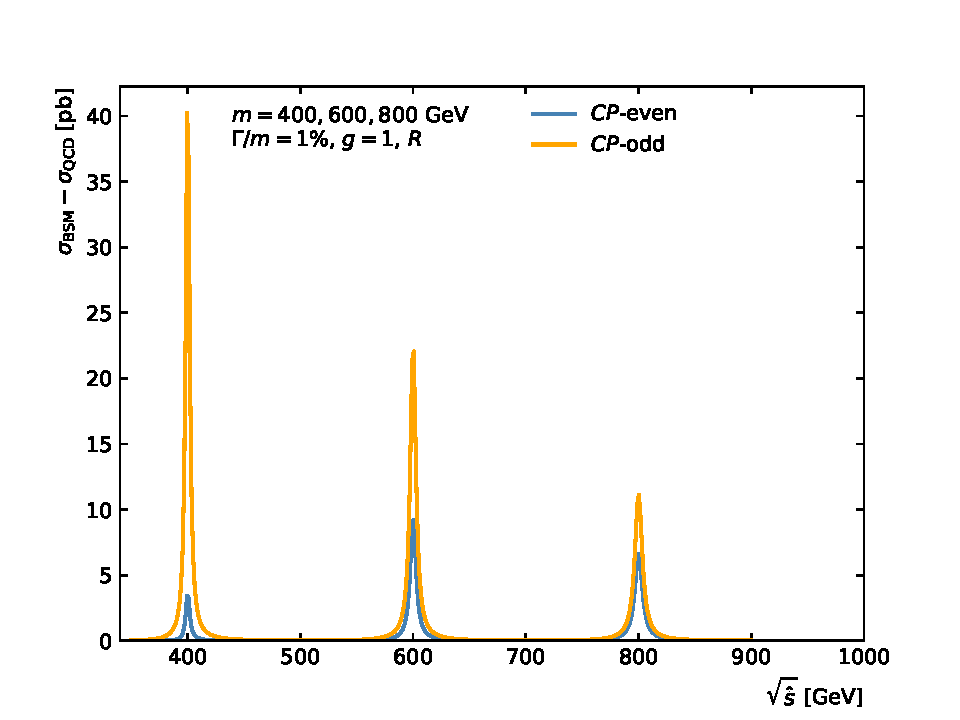
\includegraphics[width=0.49\textwidth]{fig/chapt4/gen_plots/analytical/xSec_relW1_R}
  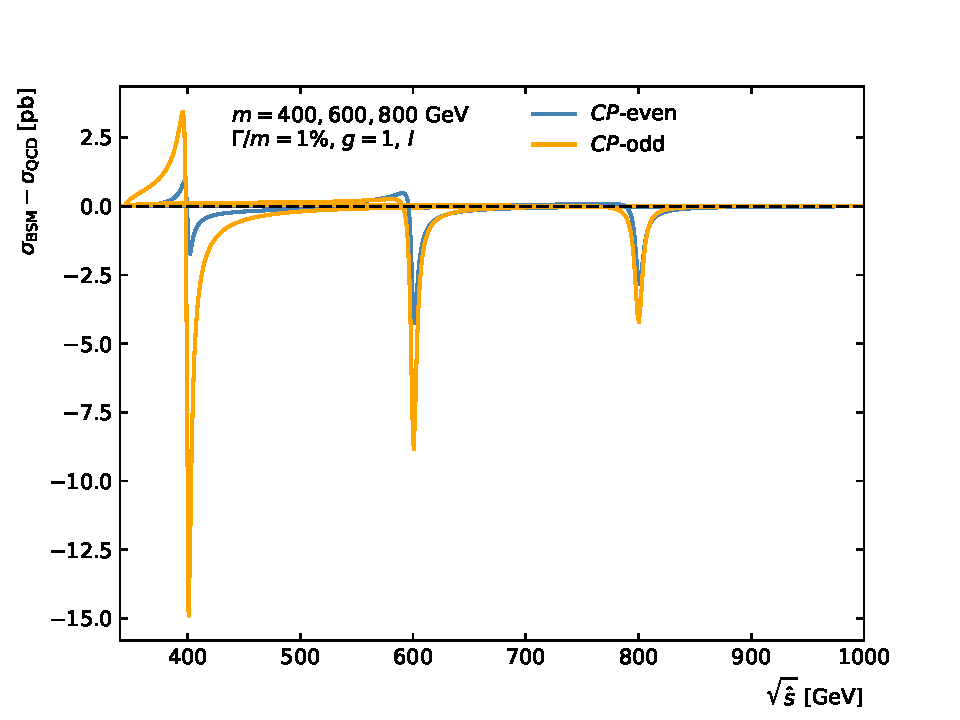
\includegraphics[width=0.49\textwidth]{fig/chapt4/gen_plots/analytical/xSec_relW1_I} \\
  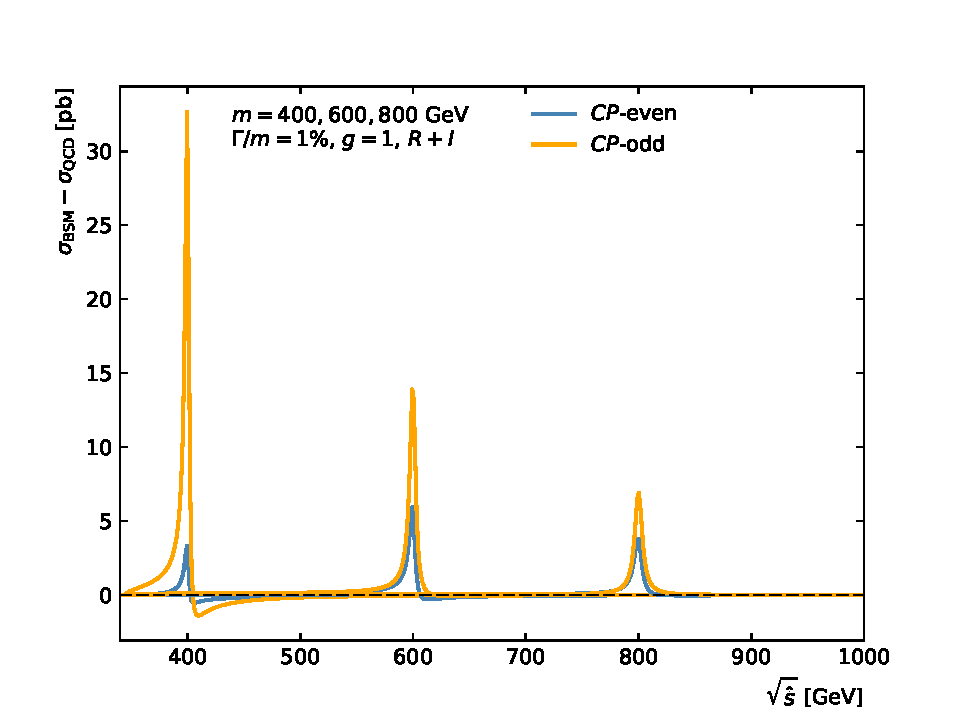
\includegraphics[width=0.49\textwidth]{fig/chapt4/gen_plots/analytical/xSec_relW1_Sum}
  \caption{Parton-level cross sections for the resonant part of the signal (upper left), the interference (upper right), and the sum of the two (bottom) for a total width of 1\%.}
  \label{Fig:AnalyticXSec_relW1}
\end{figure}

\begin{figure}
  \centering
  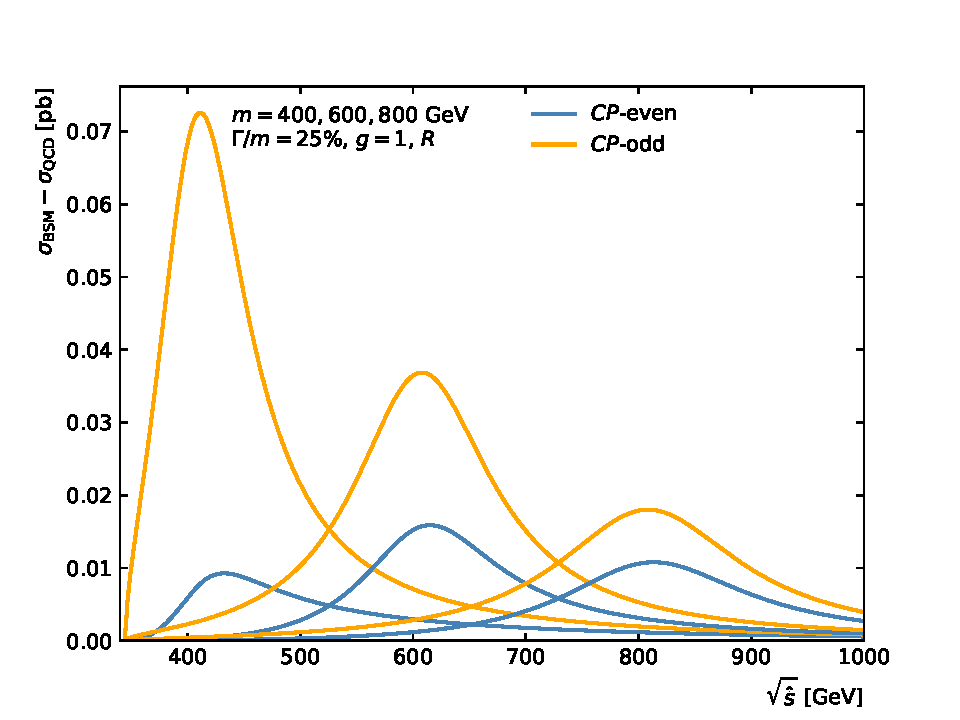
\includegraphics[width=0.49\textwidth]{fig/chapt4/gen_plots/analytical/xSec_relW25_R}
  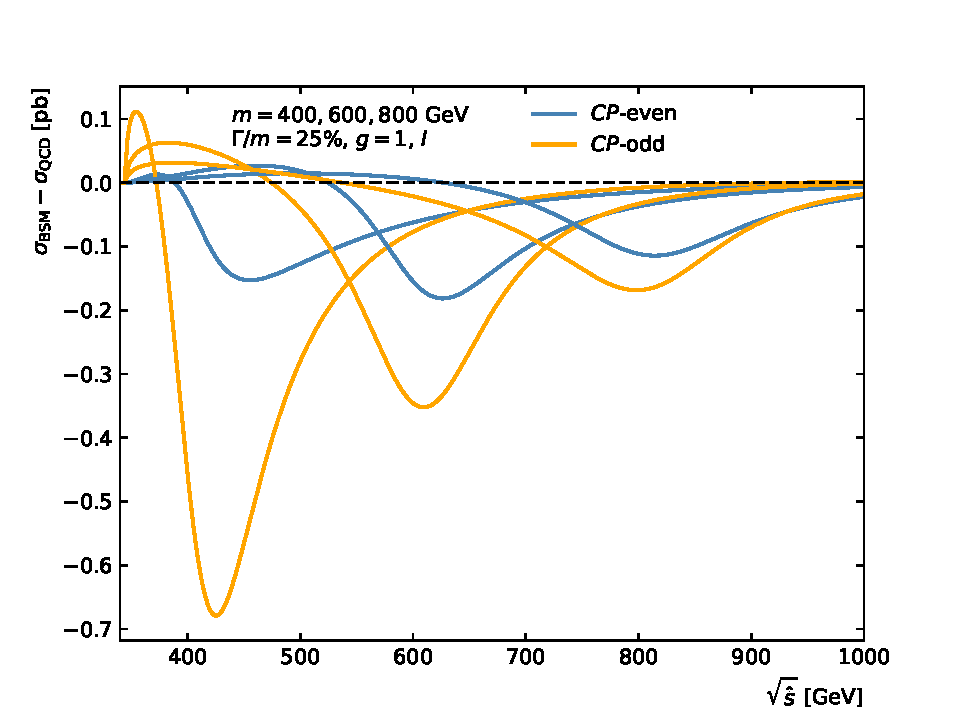
\includegraphics[width=0.49\textwidth]{fig/chapt4/gen_plots/analytical/xSec_relW25_I} \\
  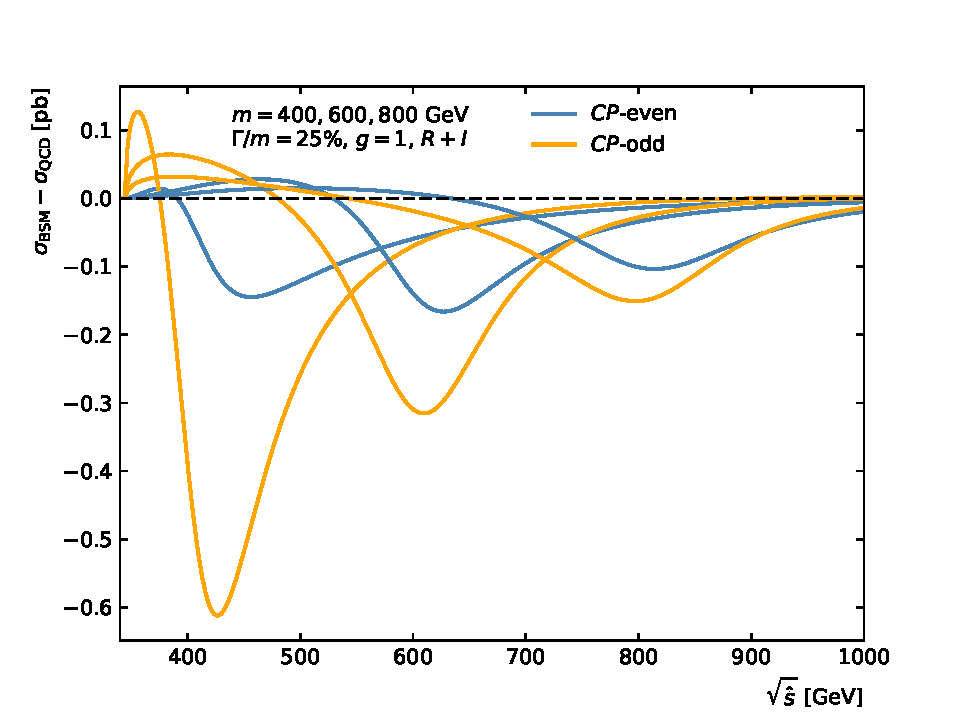
\includegraphics[width=0.49\textwidth]{fig/chapt4/gen_plots/analytical/xSec_relW25_Sum}
  \caption{Parton-level cross sections for the resonant part of the signal (upper left), the interference (upper right), and the sum of the two (bottom) for a total width of 25\%.}
  \label{Fig:AnalyticXSec_relW25}
\end{figure}



\clearpage{\pagestyle{empty}\cleardoublepage}
\renewcommand*{\thesection}{\thechapter.\arabic{section}}       % reset again to chaptnum.sectnum